\chapter{Introduction}

In this chapter we present the main features of a turbulent flow, providing an historical background of the direct numerical simulation field applied to the channel flow problem.

\section{Turbulent flows}
Every smoker can observe the nature of turbulence one inch away from their nose.
However a proper definition of turbulence is not yet given, due to the complexity of turbulence behaviour. \par
To use Prandtl words, who began an important lecture as follows: \\~\\
\emph{``What I am about to say on the phenomena of turbulent flows is still far from conclusive. It concerns, rather, the first steps in a new path which I hope will be followed by many others. The researches on the problem of turbulence which have been carried on at G\"{o}ttingen for about five years have unfortunately left the hope of thorough understanding of turbulent flow very small. The photographs and kinetographic pictures have shown us only how hopelessly complicated this flow is.''} \\~\\

Nowadays we can entrust to computational units that allows us to be no longer \emph{``hopeless''} as Prandtl was, although we are still far from having a solution, or at least a unique definition, of what the turbulence is. 
At the present time we define the turbulence as a flow regime, characterized by high Reynolds numbers and the presence of high level of diffusivity and irregularity, dissipation and three dimensional chaotic fluctuations in space and time\cite{turbulence:def}.


\section{General concepts}
An elderly definition of turbulence was provided by Hinze~\cite{Hinze}, in 1959, and say:\\~\\
\emph{``Turbulent fluid motion is an irregular condition of flow in which the various quantities show a random variation with time and space coordinates, so that statistically distinct average values can be discerned''}.\\~\\
The concept of \emph{average} is the keyword that humanity has used to start digging into the turbulence mysteries.
This kind of process, with its high sensitivity to the boundaries and initial conditions, can be defined as chaotic, so it can not be treated with a deterministic approach, therefore such randomness can be handled only by using a statistical approach.
In fact turbulence recovers its deterministic side inside statistical analysis: the detailed properties of the signal show a non predictable behaviour, but its statistical properties are consistent~\cite{Frisch}.
At statistical level, turbulent phenomena become reproducible and subject to systematic study, providing a basis for theoretical description. Therefore, the three-dimensional time-dependent Navier-Stokes equations can be solved and then the solution is averaged in order to obtain the statistics~\cite{Durbin}. 
\par
Note, however, that irregular motion and chaotic advection do not guarantee turbulence. Small point vortices can advect themselves in a chaotic manner or particles can follow complex trajectories, yet this is not turbulence. The definition, in fact, requires diffusivity. If the flow pattern looks random but does not exhibit high mix of momentum, mass and heat, it is surely not turbulent. Diffusivity is the single most important feature of turbulence, as highlighted by the experiment of Osborne Reynolds~\cite{Reynolds}, in 1883.
\par
In its famous work Reynolds has defined a ratio among inertia forces and viscous forces:
\begin{equation}
Re = \frac{ul}{\nu}
\end{equation}
\begin{figure}
\begin{center}
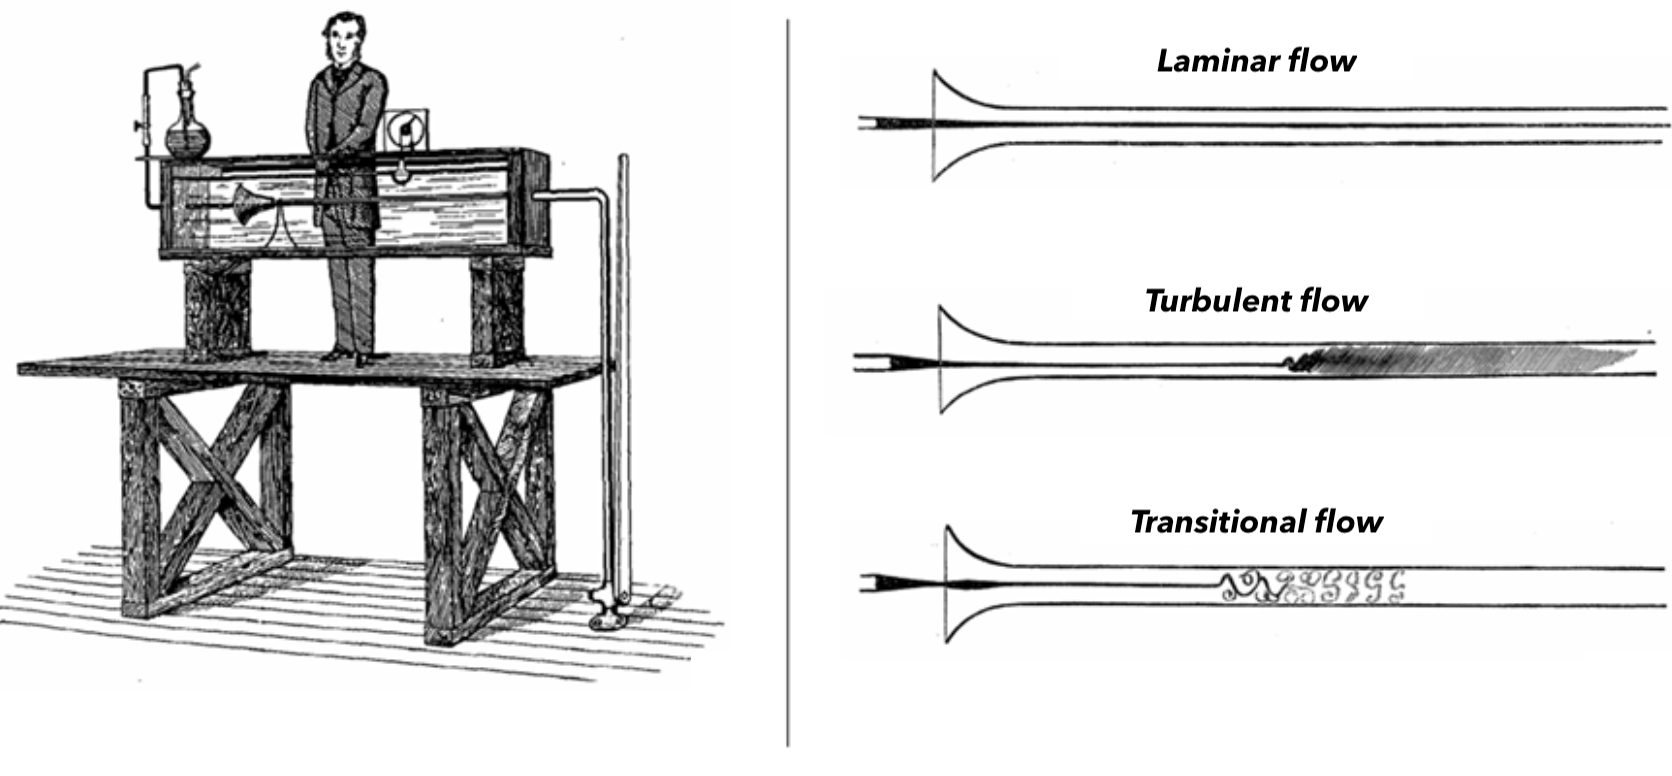
\includegraphics[width=1\textwidth]{grafici/reynolds_exp}
\caption{Sketch of the Reynolds experiment (\emph{left}) and flow patterns (\emph{right})}
\label{Reynolds:exp}
\end{center}
\end{figure}

with $u$ that is the characteristic velocity of the fluid, $l$ is the reference length of the scale and $\nu$ is the kinematic viscosity; able to predict the presence, or not, of the turbulence. He saw that when the inertia forces are huge the flow become unstable and the ink of its experiment started mixing with the surrounding water, as shown in the sketch of figure~\ref{Reynolds:exp}.
\par
This first work has correlated the presence of different states of the flow, laminar, transitional and turbulent, and their relationship with the couple viscous term-nonlinear inertia term.
Further observations revealed the presence of three-dimensional eddies. Although we are still unable to determine their shapes, we have understood that they play a key role in the turbulence sustenance. Under the assumptions of incompressible flow, not subjected to external forces of volume or surface, the vorticity equation states
\begin{equation}
\frac{D \boldsymbol{\omega}}{D t} = (\boldsymbol{\omega} \cdot \boldsymbol{\nabla})\boldsymbol{u} + \nu \boldsymbol{\nabla}^{2} \boldsymbol{u}.
\end{equation}
The central term of the equation, $ (\boldsymbol{\omega} \cdot \boldsymbol{\nabla})\boldsymbol{u}$, is known as vortex-stretching term. 
The vortex stretching is at the core of the description of the turbulent energy cascade, from the large scales to the smallest scale, determined, as we will see, by the turbulence itself.
For incompressible flow, due to volume conservation of fluid elements, the lengthening implies thinning of the fluid elements in the directions perpendicular to the stretching direction. This reduces the length scale of the associated vorticity. Finally, at the smallest scales the turbulence kinetic energy is dissipated into heat through the action of molecular viscosity~\cite{Lumley}.



\section{The history of the direct numerical simulation}
The direct numerical simulation (DNS) of the Navier-Stokes equations is a mathematical tool used to analyze turbulent flows since it allows to have an inner viewpoint in the transition and turbulence phenomena processes. It is part of the so called Computation Fluid Dynamics, or CFD, research field. 
Given the high computational cost of these simulations, DNS is not used to reproduce real-life flows, but as a research tool for flows with simple boundaries\cite{dns:tool}. \par
Despite of such kind of simulations, due to their limits, could seem useless, they assume relevant importance in the study of the turbulence, who, dominating the small scales, affect the behavior of the large scales, determining the raise of phenomenas such as flow separations, drag increases or losses of lift.
These simulations rely on high accuracy computational methods and they do not employ turbulence models, hence they require an ever-increasing computational power, as we move towards engineering relevant Reynolds numbers. 
However we can identify an ultimate threshold for direct numerical simulation of the wall bounded flows, which, thanks to its scale separation,  give the possibility to model the turbulence phenomena once for all. In~\cite{Jimenez2003} professor Jiménez set such threshold around $Re_{\tau}=10000$.\\~\par




The DNS history is recent, with the first milestone work carried out by Kim, Moin and Moser~\cite{kim_moin_moser} in the 1987, using a $192\times 129 \times160$ grid of points distributed in a channel flow domain, in which they studied the homogenous isotropic turbulence using spectral modes. Follow this seminal work other authors proposed their simulations.
Accurate DNS calculations of the turbulent channel flow, using spectral methods, have been carried out by Lyons \emph{et al.}~\cite{Lyons}, Antonia \emph{et al.}~\cite{antonia_teitel_kim_browne_1992}, Kasagi \emph{et al.}~\cite{Kasagi}, Rutledge and Sleicher~\cite{Rutledge} in the first nineties. In the 1999 Moser \emph{et al.}~\cite{KMMans} proposed their $Re_{\tau}=590$ simulation, while to see the first channel flow simulation using finite differences we have to wait Abe \emph{et al.}~\cite{Abe} in 2001.\par
Other works, from the first years of the twenty-first century, are for example Iwamoto \emph{et al.}~\cite{Iwamoto} ones, Del Alamo and Jiménez~\cite{delalamo} and, the first simulation with $Re_{\tau}$ over a thousand, Del Alamo \emph{et al.}~\cite{delalamo2} work, in 2004. \par
Between 2004 and 2007 were presented different works, alternating the finite differences techniques with the more established spectral methods approach.
Tanahashi \emph{et al.}~\cite{Tanahashi}, Iwamoto \emph{et al.}~\cite{Iwamoto2}, Hoyas and Jiménez~\cite{Hoyas}, Hu \emph{et al.}~\cite{Hu}are some examples. \par
More recent simulation have been carried out by Lozano-Duràn \emph{et al.}~\cite{Lozano}, Lozano-Duràn and Jiménez~\cite{Lozano2}, Vreman and Kuerten~\cite{Vreman}, Bernardini \emph{et al.}~\cite{Bernardini} and the actually biggest simulation ever, with $Re_{\tau}=5200$, by Lee and Moser~\cite{Lee}. \par

\begin{figure}
\begin{center}
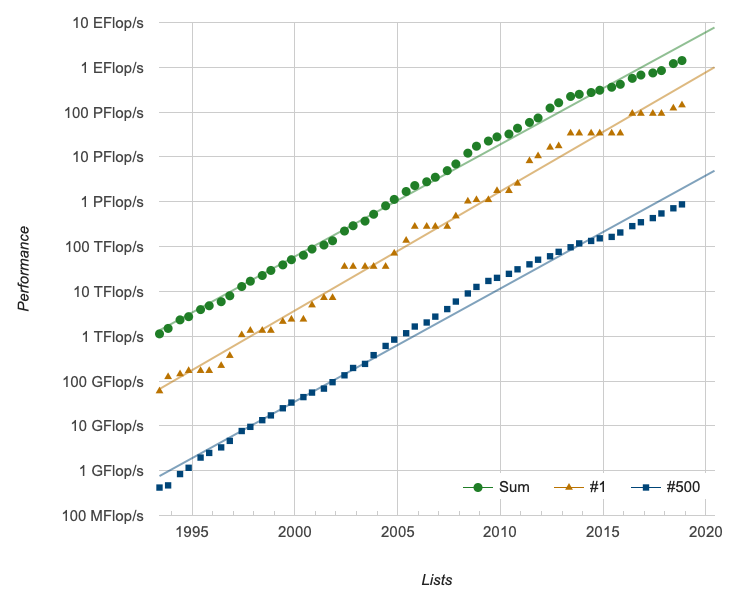
\includegraphics[width=0.8\textwidth]{grafici/top500hist}
\caption{Supercomputers grown trend, courtesy of TOP500.org}
\label{top500}
\end{center}
\end{figure}
\begin{figure}
\begin{center}
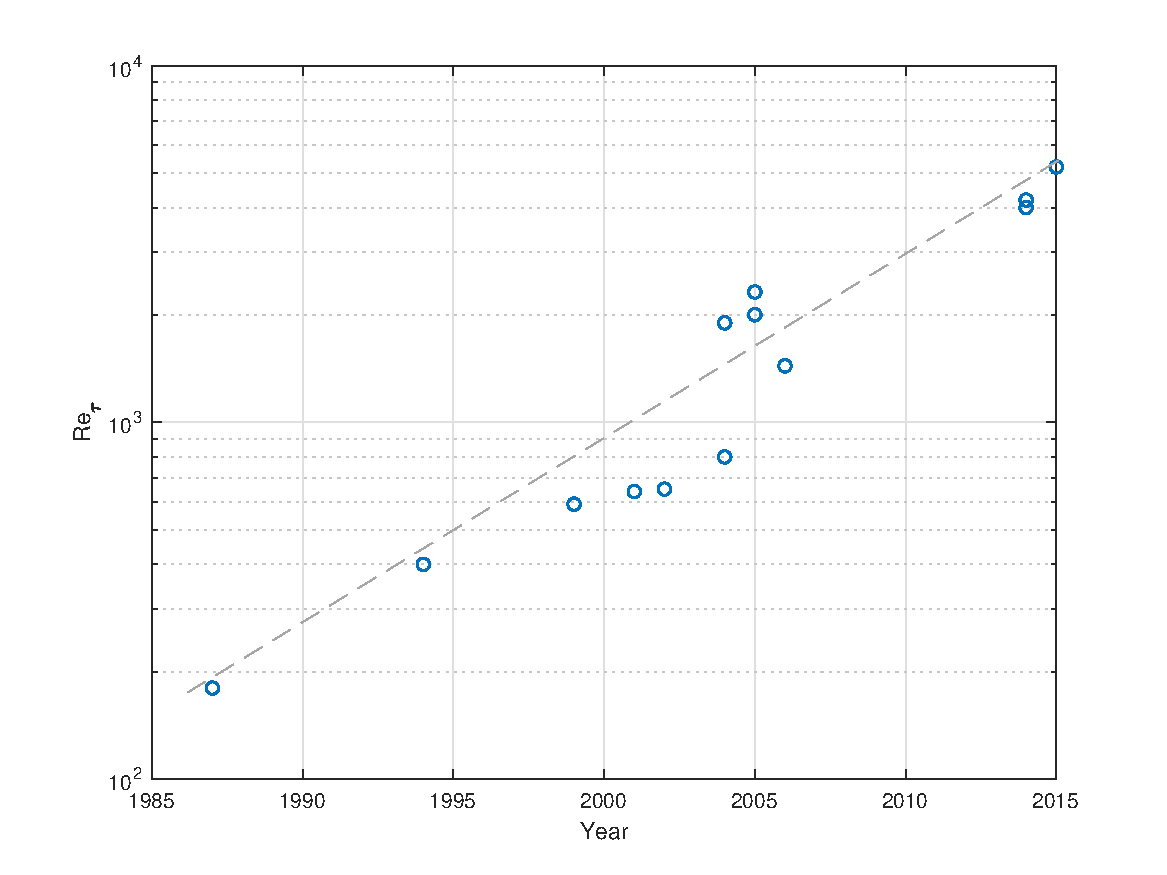
\includegraphics[width=0.8\textwidth]{grafici/dns_trend}
\caption{$Re_{\tau}$ growth trend}
\label{dns:trend}
\end{center}
\end{figure}

The grows in $Re_{\tau}$ number is correlated with the grown in supercomputing performances on those years, as could be understood by looking at figures~\ref{top500} and~\ref{dns:trend}. However the $Re_{\tau}$ growth is not proportional with the computational power, as we can clearly see. \par
We are not far from the possibility to solve the biggest useful simulation, in~\cite{Jimenez2003} is reported that a theoretical 500 Pflops supercomputer could carry out the $Re_{\tau}=10000$ simulation in a reasonable time. The cited document has been published in 2003, but, unfortunately, starting from 2013, the rate of growth of the supercomputers speed has halved with respect to the past decade, and this made the forecast embedded in such document wrong. However, with the current rate of growth, it is likely that we could carry out such simulation within the next three years. \\~\par

In this thesis our goal was to provide an highly parallelized DNS solver, based on pseudo-spectral approach, able to carry out simulation on a wide number of processors in an efficient way. \par
We were particularly interested in the possibility to generate flow statistics at high $Re_{\tau}$ values, in reasonable time, maintaining code efficiency above the~40\%. \\~\par




  




  